\section{La función de reproducción humana}

La función de reproducción humana permite que las personas adultas puedan tener descendientes, es decir, hijas o hijos. La lleva a cabo el \textbf{aparato reproductor}.

\vspace{3mm}
\textbf{Nuestra reproducción es sexual}; es decir, que para tener lugar deben intervenir dos células reproductoras de distinto sexo: los \textbf{espermatozoides} y los \textbf{óvulos}. Estos dos tipos de células son producidas, respectivamente, por uno de los \textbf{dos tipos de aparato reproductor} que existen.

\vspace{3mm}
\textbf{La producción de espermatozoides} (Figura \ref{fig:reproductor-masculino})

\vspace{3mm}
El aparato reproductor que \textbf{se encarga de la producción de los espermatozoides}, es el que puedes ver a continuación:

\begin{figure}[!ht]
    \centering
    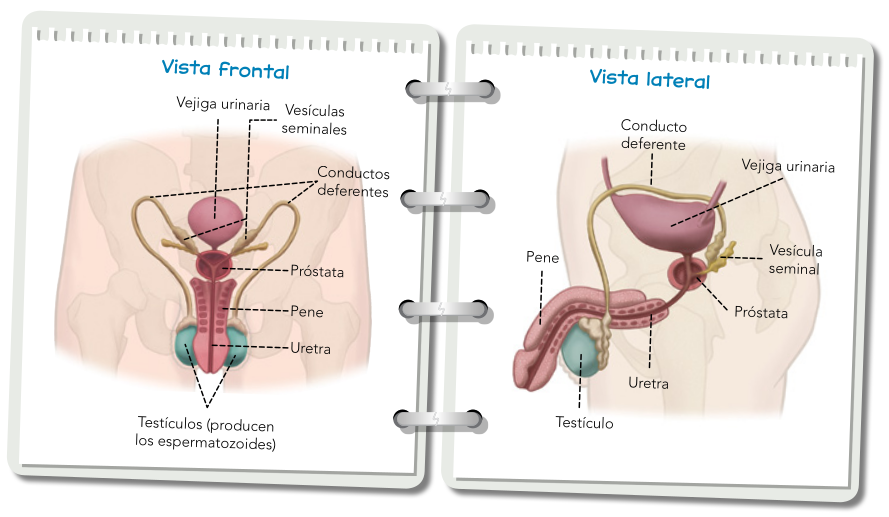
\includegraphics[width=0.7\linewidth]{Tema3/15_Aparato_reproductor_masculino.png}
    \caption{Aparato reproductor masculino}
    \label{fig:reproductor-masculino}
\end{figure}

\textbf{La producción de óvulos} (Figura \ref{fig:reproductor-femenino})

\vspace{3mm}
El aparato reproductor que \textbf{se encarga de la producción de los óvulos} es el que puedes ver en las imágenes de esta página. Además, está preparado para que en su interior tengan lugar la unión de las células reproductoras y el desarrollo del nuevo ser desde sus primeras etapas hasta su nacimiento.

\begin{figure}[!ht]
    \centering
    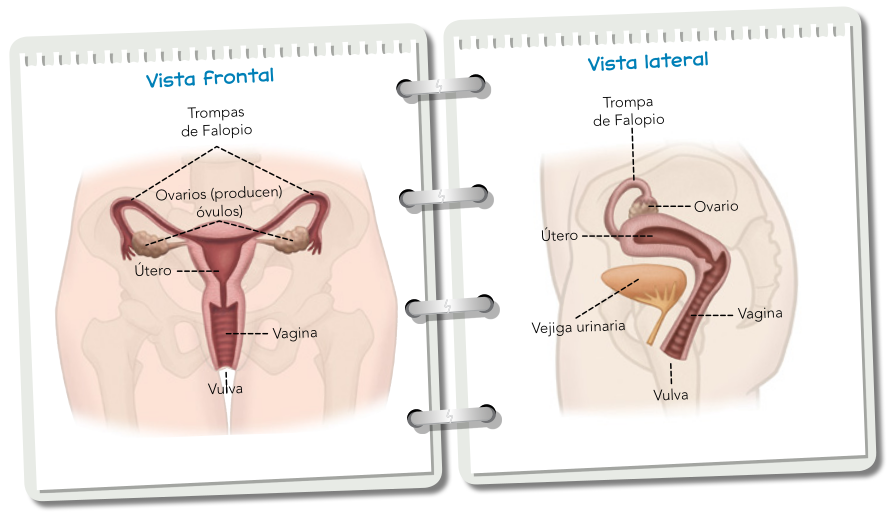
\includegraphics[width=0.7\linewidth]{Tema3/16_Aparato_reproductor_femenino.png}
    \caption{Aparato reproductor femenino}
    \label{fig:reproductor-femenino}
\end{figure}

\textbf{La pubertad}

\vspace{3mm}
Aunque nacemos con aparato reproductor, este no está completamente activo hasta cierta edad. Ese momento, que se produce entre los 10 y los 16 años, es el comienzo de la \textbf{pubertad}.

\begin{itemize}
    \item \textbf{Pubertad y producción de espermatozoides}. Cuando los testículos comienzan a producir espermatozoides, también segregan hormonas que causan la aparición del vello púbico y de la barba, el cambio del tono de voz, el desarrollo de una forma corporal más adulta...
    \item \textbf{Pubertad e inicio del ciclo menstrual}. Ocurre cuando los ovarios empiezan a liberar óvulos maduros, de uno en uno, más o menos cada 28 días. Esta liberación se llama \textbf{ovulación}. Es ahora cuando aparece la primera \textbf{regla o menstruación} y cuando se inicia la producción de hormonas que causan el desarrollo de vello púbico, de las mamas...
\end{itemize}

\subsection{El proceso de la reproducción}

El proceso de la reproducción en los seres humanos tiene lugar en tres fases: la \textbf{fecundación}, el \textbf{embarazo} y el \textbf{parto}.

\subsubsection{La fecundación}

La fecundación es la unión de las dos células reproductoras, el óvulo y el espermatozoide, para formar el cigoto, que es la célula que se desarrollará para formar el nuevo ser.

\vspace{3mm}
La fecundación suele tener lugar en el interior de las trompas de Falopio, mientras el óvulo está descendiendo desde el ovario que lo liberó. Sucede cuando un espermatozoide consigue entrar en el óvulo y los dos núcleos celulares se combinan.

\subsubsection{El embarazo}

El embarazo es el período que transcurre desde que se forma el cigoto hasta el nacimiento del bebé. Dura unos nueve meses y en él se producen numerosos cambios:

\vspace{3mm}
\textbf{El primer trimestre}

\vspace{3mm}
Tras la fecundación, el cigoto comienza a dividirse en varias células. Esto origina un \textbf{embrión}, que \textbf{se implanta} en el revestimiento de la pared del útero, llamado endometrio.

\vspace{3mm}
Poco después, alrededor del embrión se forma una membrana llena de líquido, el \textbf{saco amniótico}, donde queda protegido.

\vspace{3mm}
Al mismo tiempo se forma la \textbf{placenta}, que es un órgano que se conecta directamente a los vasos de la pared de útero. La placenta intercambia sustancias entre la sangre de la madre y el embrión a través del \textbf{cordón umbilical}.

\vspace{3mm}
\textbf{El segundo trimestre}

\vspace{3mm}
\textbf{El embrión pasa a llamarse feto}, crece y en él \textbf{comienzan a formarse casi todos los órganos}. Poco a poco adquiere un aspecto humano y comienza a realizar movimientos.

\vspace{3mm}
\textbf{El tercer trimestre}

\vspace{3mm}
\textbf{El feto prosigue su maduración y crecimiento}. A partir del séptimo mes, el desarrollo corporal es completo, aunque los pulmones o el aparato digestivo aún no están maduros. Hacia el noveno mes, el feto \textbf{se encaja}, es decir, se coloca con la cabeza hacia la salida del útero, preparándose para nacer.

\begin{figure}[!ht]
    \centering
    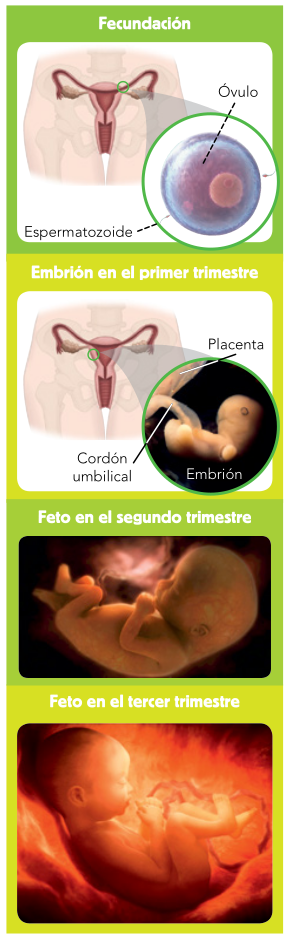
\includegraphics[width=0.3\linewidth]{Tema3/17_Proceso_reproduccion.png}
    \caption{El proceso de la reproducción}
    \label{fig:proceso-reproduccion}
\end{figure}

\subsubsection{El parto}

Cuando se acerca el momento del parto, \textbf{las paredes del útero comienzan a contraerse. El cuello del útero y la vagina se dilatan} para permitir la salida del feto.

\vspace{3mm}
Finalmente, \textbf{el saco amniótico se rompe} y el bebé y la placenta son expulsados al exterior. Los pulmones se activan y el bebé comienza a respirar.

\vspace{3mm}
Tras el nacimiento, el cordón umbilical debe ser cortado. El \textbf{ombligo} es la cicatriz que queda en el lugar del abdomen en el que el cordón estaba conectado al feto.

\vspace{3mm}
Como ocurre con otros mamíferos, \textbf{los bebés humanos están preparados para alimentarse de la leche que producen las mamas de la madre}. En esos primeros meses de vida continúa la maduración de su aparato digestivo y del sistema nervioso, que necesitan un tiempo para estar completamente operativos.

\subsection{Reproducción y salud}

\subsubsection{Pubertad y salud}

A vuestra edad, es posible que hayáis comenzado a experimentar los cambios de la pubertad, tanto físicos como mentales. Por eso conviene tener en cuenta algunos aspectos que pueden ayudar a mantener una salud adecuada.

\begin{itemize}
    \item \textbf{Cuidar la higiene personal} es importante a cualquier edad, pues contribuye a mantener un buen estado de salud. No obstante, los cambios de la pubertad pueden implicar que necesitéis prestar más atención a la higiene de vuestra piel o de las partes externas del aparato reproductor.
    \item \textbf{Respetar y exigir respeto}. Los cambios asociados a la pubertad no suceden de igual modo y al mismo tiempo en todas las personas. Puede que en vuestro grupo haya quien aún no haya empezado a cambiar y quien ya haya experimentado la mayor parte de los cambios. En estas circunstancias es muy importante el respeto mutuo.
    \item \textbf{Decidir de forma saludable por vuestra cuenta y no dejarse arrastrar por la presión del grupo}. Coincidiendo con la pubertad, seguramente experimentéis una serie de cambios en vuestra forma de ser. Os hacéis mayores y se empieza a definir vuestra personalidad. Las amistades cobran mucha importancia y el grupo ejerce mucha influencia. Es importante que sepáis decidir y actuar según lo que pensáis, teniendo en cuenta lo que es saludable, justo o respetuoso.
\end{itemize}